\documentclass[main.tex]{subfiles}
\begin{document}

\chapter{Computer Science}
\section{计算机网络}
\subsection{TCP连接管理}
\subsubsection{TCP的三次握手}
\begin{enumerate}
    \item 客户机向服务器发送一个连接请求报文段,此报文段不含应用层数据,SYN=1,客户端会选择一个随机的起始序seq=x。
    \item 服务端收到并同意后,发回确认,分配TCP缓存和变量,SYN=1, ACK=1,确认号为x+1,服务器随机产生起始需要seq=y,同样不包含应用层数据。
    \item 客户端收到后,向服务器发回确认,分配TCP缓存和变量,ACK=1,序号为x+1,确认号ack字段为y+1,该报文段可携带数据。
\end{enumerate}
\subsubsection{TCP的四次挥手}
\begin{enumerate}
    \item 客户机发送连接释放报文段,FIN=1, seq=u,TCP是全双工的,当发送FIN报文时,发送的那一端就不能再发送数据了,而接收的那一段此时仍可以发送数据。
    \item 服务端发送确认,确认号为u+1,此时TCP连接处于半关闭状态,服务端发送数据,客户端仍要接收。
    \item 若服务器已经没有向客户端发送的数据,那就通知TCP释放连接,此时发送FIN=1的连接释放报文段。
    \item 客户端收到连接释放报文段之后,必需发送确认,ACK=1, seq=u+1,此时TCP连接没有被释放掉,等待2MSL后客户端关闭连接。
\end{enumerate}

\section{人工智能}


\section{软件工程}


\section{数据库系统原理}
\subsection{绪论}
\subsubsection{基本概念}
数据是数据库中存储的基本对象,数据与其语义是不可分的,语义即对数据含义的说明。数据库是长期存储在计算机内、有组织的、可共享的大量数据的集合。\\
DBMS的主要功能如下:\\
\begin{enumerate}
    \item 提供数据定义语言DDL,定义数据对象。
    \item 提供数据操纵语言DML,实现对数据库的增删改查。
    \item 实现数据的组织、存储和管理,分类组织、确定数据的文件结构和存取方式,实现数据之间的联系。
    \item 数据库的运行管理。
    \item 数据库的建立和维护。
\end{enumerate}
DBS数据库系统:在计算机系统中引入数据库后的系统构成。有如下构成:数据库、数据库管理系统、应用系统、数据库管理员。数据结构化、共享性高、冗余度低且独立性高。其中的数据由DBMS统一管理和控制。数据独立性是由DBMS的二级映像功能来保证的。\\
DBAS数据库应用系统:就相当于计算机应用系统,是数据库系统与用户应用程序的结合,例如财务软件等等。\\
在数据库中使用数据模型来抽象、表示和处理现实世界中的事物。其组成要素有:数据结构、数据操作和完整性约束。数据模型分为概念模型、逻辑模型和物理模型。概念模型,即按用户的观点对数据和信息的建模,用于数据库设计。逻辑模式包括网状模型、层次模型、关系模型等,是按计算机系统的观点对数据建模,用于DBMS的实现。物理模型是对数据最底层的抽象,即在磁盘或磁带上的存储方式和存取方法。\\
在E-R图中,用矩形表示实体名(比如学生),用椭圆表示属性(比如姓名和学号),用菱形来表示联系,菱形框内写明联系名,然后在无向边中标注联系的类型。其中联系也可以具有属性:
\begin{figure}[H]
    \centering
    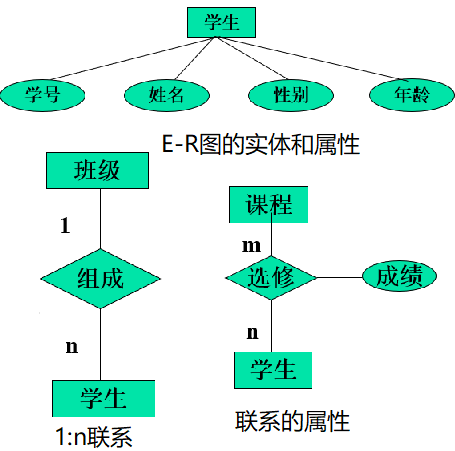
\includegraphics[scale=0.8]{./images/0019.png}
    \caption{E-R图的表示}
\end{figure}
\subsubsection{数据模型}
\begin{enumerate}
    \item 格式化模型
        \begin{enumerate}
            \item 层次模型:以树形结构来表示实体和实体间的联系,如图,其也有根节点和叶子结点等等,其只能直接处理一对多的实体联系,任何记录只有按其路径查看时,才能显示出其全部的意义,子女记录不能脱离双亲记录而单独存在。如果是多对多的话,需要将多对多分拆成多个一对多然后用层次模型表示。其查询效率高,性能优于关系模型,且不低于网状模型。
                \begin{figure}[H]
                    \centering
                    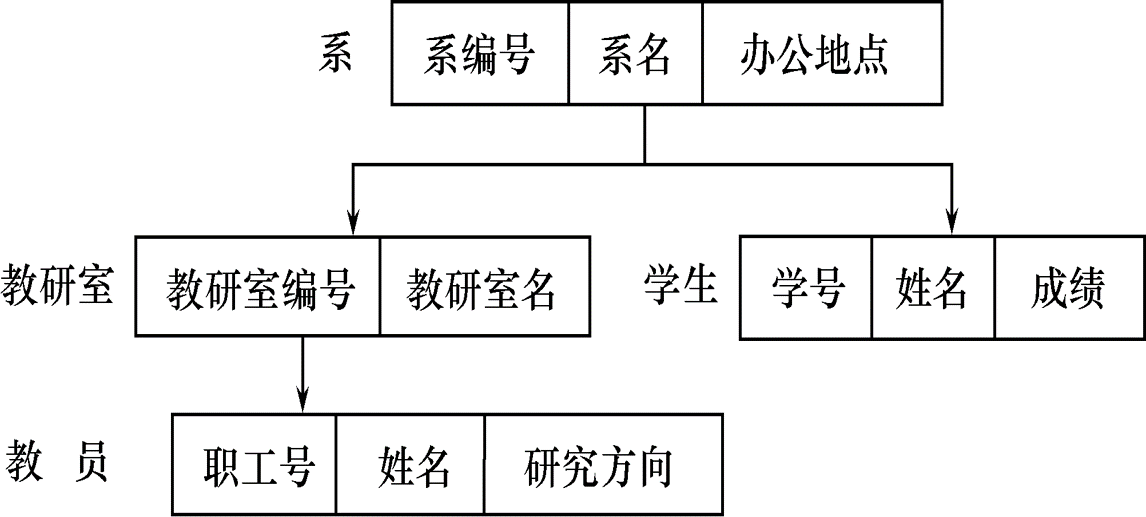
\includegraphics[scale=0.5]{./images/0020.png}
                    \caption{层次模型}
                \end{figure}
            \item 网状模型:允许一个以上的结点无双亲,且一个结点可以有多于一个的双亲。由此可见,层次模型实际上是网状模型的一个特例。网状模型的结构比较复杂,随着应用环境的扩大,数据库结构就变得愈发复杂,不利于用户的最终掌握。如下图:
                \begin{figure}[H]
                    \centering
                    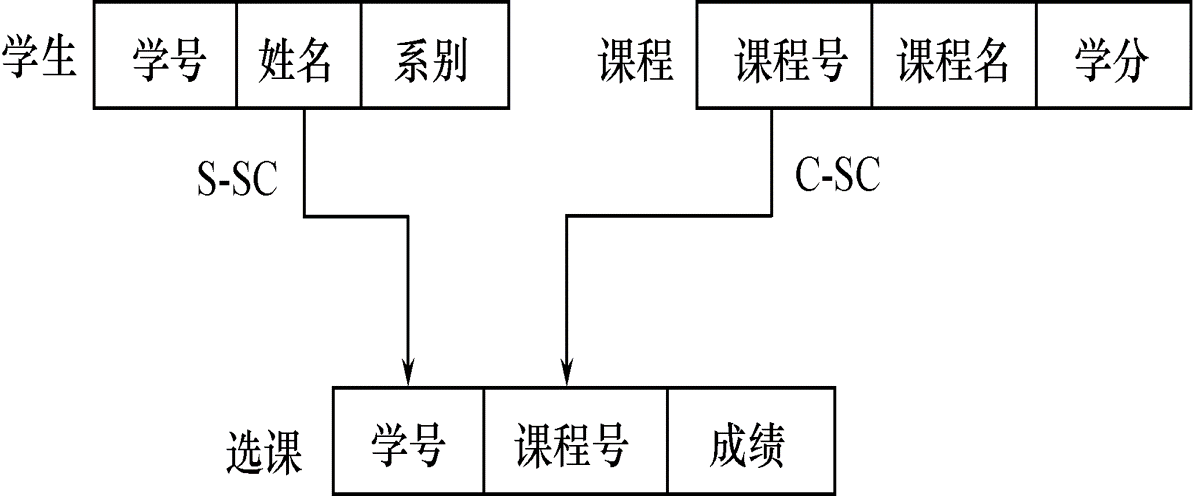
\includegraphics[scale=0.5]{./images/0021.png}
                    \caption{网状模型}
                \end{figure}
        \end{enumerate}
    \item 关系模型:关系模型下数据的逻辑结构是一张二维表,由行和列组成。其中,关系必须是规范化的,每一个分量必须是一个不可分的数据项,不允许表中有表。例如下图中的工资就是一个可分的数据项,所以其不符合关系模型的要求。关系模型中实体和各类的联系都用关系来表示,其概念单一,可描述一对一、一对多和多对多的联系,具有更高的数据独立性。
        \begin{figure}
            \centering
            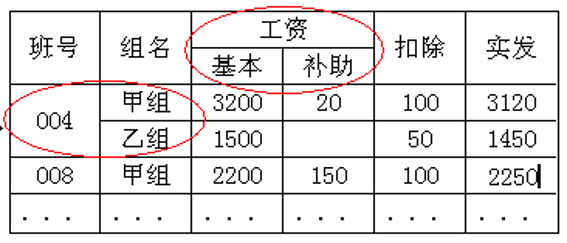
\includegraphics[scale=0.5]{./images/0022.png}
            \caption{表中有表的实例}
        \end{figure}
\end{enumerate}
\subsubsection{数据库的系统结构}
提到了一种叫做模式(schema)的概念,一般说的模式,指的是逻辑模式,是对数据库中全体数据的逻辑结构和特征的描述。{\bfseries 一个数据库只有一个模式}。


\section{编译原理}

\end{document}
